\documentclass[journal,11pt,twocolumn]{IEEEtran}

\usepackage{enumitem}
\usepackage{amsmath}
\usepackage{amssymb}
\usepackage{graphicx}
\providecommand{\pr}[1]{\ensuremath{\Pr\left(#1\right)}}
\providecommand{\cbrak}[1]{\ensuremath{\left\{#1\right\}}}
\providecommand{\cdf}[2]{\ensuremath{F_{#1}\left(#2\right)}}

\title{Assignment 3}
\author{Velma Dhatri Reddy \\ \normalsize AI21BTECH11030 \\ \vspace*{10pt} \Large CBSE Probability Grade 10}
\begin{document}
\maketitle
\textbf{Exercise 15.1 Q13:}
A die is thrown once. Find the probability of getting	\begin{enumerate}[label=(\roman*)]
		\item a prime number
		\item a number lying between 2 and 6
		\item an odd number
\end{enumerate}

\textbf{Solution:} Let the random variable $X$ denote the number that appears on rolling the die. The sample space is $S = \cbrak{1, 2, 3, 4, 5, 6}$. The CDF can be obtained from the PMF as follows:

\begin{align}
    \cdf{X}{k} = \sum_{i = 1}^{i = k}\pr{X = i} = k \times \frac{1}{6} = \frac{k}{6}
\label{cdf}
\end{align}

Hence, using Fig.\ref{fig:pmf-cdf}

\begin{enumerate}[label=(\roman*)]

	\item The probability of getting a prime number  
	
\begin{align}
    &= \pr{X=2} + \pr{X=3} + \pr{X=5}\\
    &= 3\times \dfrac{1}{6}\\
    &= \dfrac{3}{6}\\
    &= 0.5
\end{align}

	\item The probability of getting a number lying between 2 and 6 is
	
\begin{align}
    \pr{2 < X \leq 5} &= \cdf{X}{5} - \cdf{X}{2}\\
    &= \dfrac{5}{6} - \dfrac{2}{6}\\
    &= \dfrac{3}{6}\\
    &= 0.5
\end{align}

	\item The probability of getting an odd number
	
\begin{align}
    &= \sum_{i = 0}^{i = 2}\pr{X = 2\times i + 1}\\
    &= 3\times \dfrac{1}{6}\\
    &= \dfrac{3}{6}\\
    &= 0.5
\end{align}

\end{enumerate}

\begin{figure}[!ht]
\centering
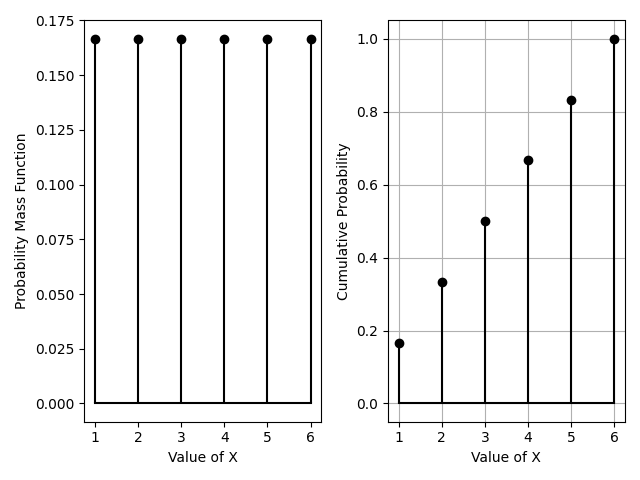
\includegraphics[width=\columnwidth]{figs/3_1.png}
\caption{Plot of the PMF (left) and CDF (right) of an unbiased die}
\label{fig:pmf-cdf}
\end{figure}

\end{document}